% !TEX root = ../master-thesis.tex




Precise control over the depth of each optical tweezer is essential for preparing few-fermion systems via spilling techniques. In our setup, each tweezer is initially loaded with approximately \red{100} atoms, which are then selectively removed by ramping down the potential depth. The number of remaining atoms as a function of spill power $x_{\mathrm{sp}}$ exhibits a quantized staircase structure, reflecting the discrete energy levels of the 1D harmonic oscillator. This behavior can be characterized by a step plot~\cite{holten_pauli_2022}.

% \textbf{Step plot.}
To characterize this behavior in our tweezer array, we measure step plots for all sites simultaneously. Figure~\ref{fig:stepplot}a shows the result for a $4 \times 4$ array. For each value of $x_{\mathrm{sp}}$, we acquire 70 experimental realizations and compute the average photon signal per site. 
% This signal serves as a robust proxy for atom number. In contrast to single-atom counting, this approach is parameter-free and effective even for large initial occupancies.
% \textbf{Uniformity characterization.}
To quantify depth inhomogeneity across the array, we fit each step trace with a sigmoid function:
\begin{equation*}
    \sigmoid(x) = \frac{A_j}{1 + \exp\left(-(x - x_j)/\sigma_j\right)},
\end{equation*}
where $x_j$ denotes the center of the step and $\sigma_j$ its width for tweezer $j$. We define a relative uniformity metric as $\std(x_j) / \langle x_j \rangle$. After camera-based balancing (Sec.~\ref{subsec:control}), this metric typically yields $\sim 3\%$, which is insufficient for deterministic preparation across the array. A more precise balancing procedure is therefore required.




% \textbf{Single-value feedback.}
To further improve uniformity, we apply an iterative atom-based feedback scheme. Rather than fitting full step plots, we operate at a single point on the slope of the transition, near the half-filling level $A_j / 2$. At this point, the sigmoid can be approximated by a linear response:
\begin{equation*}
    \sigmoid(x) \approx \frac{A_j}{4 \sigma_j} x - \frac{A_j x_j}{4 \sigma_j},
\end{equation*}
assuming $x_j \gg \sigma_j$.  In the feedback loop, we do not use the fitted sigmoid parameters directly. Instead, we measure a single photon-count matrix $M_{ij}$ and treat it as a linear proxy for the power matrix $P_{ij}$. Since the sigmoid offset $\mathrm{shift} = A_j x_j / (4 \sigma_j)$ is known from the fits, we approximate:
\begin{equation}
    \label{mp-propto}
    M_{ij} + \mathrm{shift} \propto P_{ij} = \Lambda H_i V_j.
\end{equation}
We then factorize this matrix using the method introduced in \eqref{uv-decomposition} and update the amplitudes according to:
\begin{equation*}
    h \rightarrow h + \gamma (H - H_0), \qquad
    v \rightarrow v + \gamma (V - V_0),
\end{equation*}
where $(H_0, V_0)$ is the target point, and $\gamma$ is the feedback rate. This model-free procedure avoids full sigmoid fitting and operates directly on experimental measurements.

Figure~\ref{fig:stepplot}b shows the result of applying this single-value feedback (SVF) protocol to a $4 \times 4$ array. After five iterations, the relative deviation of the fitted step centers is reduced to $0.7(2)\%$, well within the plateau width (typically $\pm5\%$), enabling deterministic state preparation across the full array.
Figure~\ref{fig:svf}a shows the process of applying the SVF protocol to a $6 \times 6$ array. The proportionality coefficient in \eqref{mp-propto} is $A/4\sigma \sim 10(1)$ (the average value is chosen for the plot) for our experiment.




\begin{figure}
    \centering
    \addletter{170}{a}
    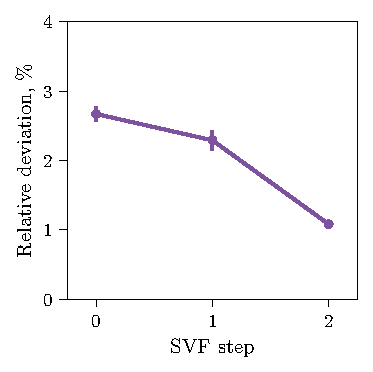
\includegraphics{fig-py/svf-avg.pdf}
    \addletter{170}{b}
    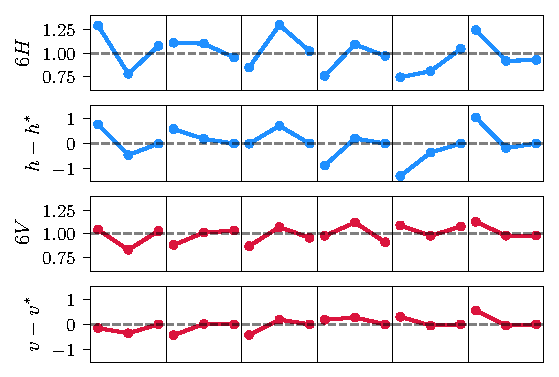
\includegraphics{fig-py/svf.pdf}
    \caption[Single-value feedback optimization for a $6 \times 6$ tweezer array]{
        \textbf{Single-value feedback (SVF) optimization for a $6 \times 6$ tweezer array.}
        (a) Relative deviation of effective powers $P_j$ across the array during successive SVF steps, quantified as $\mathrm{std}(P_j)/\langle P_j \rangle$. The initial point corresponds to camera-based balancing; subsequent iterations apply SVF with feedback rates $\gamma = 1/20$ and $\gamma = 1/40$. Further iterations did not yield statistically significant improvements. 
        (b) Retrieved horizontal powers $H_i$ and vertical powers $V_j$ (top and third rows), along with corresponding deviations of driving amplitudes from their final target values, $h - h^*$ and $v - v^*$. The recovered $H$, $V$ vectors are extracted from the photon count matrix $M_{ij}$ using factorization as described in \eqref{uv-decomposition}.
    }
    \label{fig:svf}
\end{figure}